\def\QRCODE{TB_IPR_TUT.IMG.pde_matlabqrcode.png}
\def\QRPAGE{http://www.iptutorials.science/tree/master/TB_IPR/TUT.IMG.pde/matlab}
\mcorrectionsection{Matlab correction}
%\section{Matlab correction}


\subsection{Linear diffusion}

The numerical scheme is coded as follows with matlab:
\begin{matlab}
function Z = linearDiffusion(I, nbIter, dt)
% I: Original image
% nbIter: number of iterations
% dt: step time

h = [[0 1 0];[1 -4 1];[0 1 0]];
Z=I; % initialization 

for i=1:nbIter;
    Z = Z + dt * conv2(Z, h, 'same');
end;
\end{matlab}

Another way of coding this operator is to compute 4 gradients. This simplifies the formulation of the nonlinear diffusion filter, illustrated in Fig.\ref{fig:pde:matlab:ld}.

\begin{matlab}
function Z = linearDiffusion(I,nbIter,dt)
% I: Original image
% nbIter: number of iterations
% dt: step time

% masks for gradients computation
hW = [1 -1 0];
hE = [0 -1 1];
hN = hW';
hS = hE';

Z = I; % initialization

for i=1:nbIter;
    % calculate gradient in all directions (N,S,E,W)
    gW = imfilter(Z,hW);
    gE = imfilter(Z,hE);
    gN = imfilter(Z,hN);
    gS = imfilter(Z,hS);
    
    % next Image
    Z = Z + dt*(gN + gS + gW + gE);
end;
\end{matlab}
\begin{figure}[htbp]
\centering
\subfloat[Original image.]{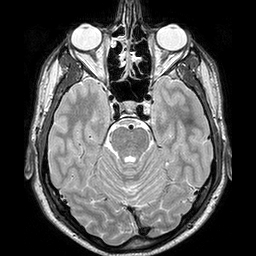
\includegraphics[width=.3\linewidth]{cerveau.png}}\hfill
\subfloat[Linear diffusion filter, with $\alpha = 0.1$,  $dt=0.05$ and 10 iterations.]{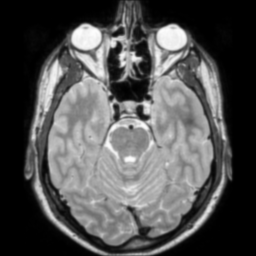
\includegraphics[width=.3\linewidth]{ld_10.png}}\hfill
\subfloat[Linear diffusion filter, with $\alpha = 0.1$, $dt=0.05$  and 50 iterations.]{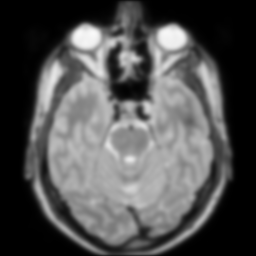
\includegraphics[width=.3\linewidth]{ld_50.png}}
\caption{Linear diffusion filter. Contours are not preserved: this is equivalent to a Gaussian filter.}
\label{fig:pde:matlab:ld}
\end{figure}

\subsection{Nonlinear diffusion}
The nonlinear diffusion is an adaptation of the diffusion to the informations contained in the images (see Fig.\ref{fig:pde:matlab:nld}). These informations are high frequency components, evaluated by the gradients in the 4 directions. A specific coefficient is thus applied to each of these directions.

\begin{matlab}
function Z = nonlinearDiffusion(I,nbIter,dt,alpha)
% I: Original image
% nbIter: number of iterations
% dt: step time
% alpha: diffusion parameter

hW = [1 -1 0];
hE = [0 -1 1];
hN = hW';
hS = hE';

Z = I;

for i=1:nbIter
    % calculate gradient in all directions (N,S,E,W)
    gW = imfilter(Z,hW);
    gE = imfilter(Z,hE);
    gN = imfilter(Z,hN);
    gS = imfilter(Z,hS);
    
    % next Image
    Z = Z + dt*(c(gN,alpha).*gN + c(gS,alpha).*gS + c(gW,alpha).*gW + c(gE,alpha).*gE);
end
\end{matlab}
with $c$ defined as follows:
\begin{matlab}
function Z = c(I, alpha)
% Perona Malik diffusion coefficient
% I: input image
% alpha: diffusion parameter
%
% absolute value is not necessary in this case
Z = exp(-(I/alpha).^2);
\end{matlab}
Another possibility is:
\begin{matlab}
function Z = c2(I, alpha)
% Perona Malik diffusion coefficient
% I: input image
% alpha: diffusion parameter
%
% absolute value is not necessary in this case
Z = 1/(1+(I/alpha).^2);
\end{matlab}

\begin{figure}[htbp]
\centering
\subfloat[Original image.]{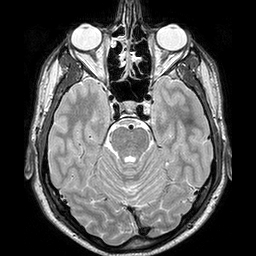
\includegraphics[width=.3\linewidth]{cerveau.png}}\hfill
\subfloat[Non linear diffusion filter, with $\alpha = 0.1$,  $dt=0.05$ and 10 iterations.]{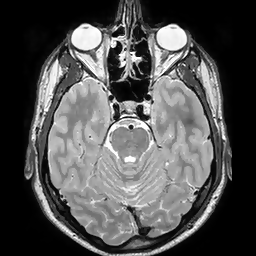
\includegraphics[width=.3\linewidth]{nld_10.png}}\hfill
\subfloat[Non linear diffusion filter, with $\alpha = 0.1$, $dt=0.05$  and 100 iterations.]{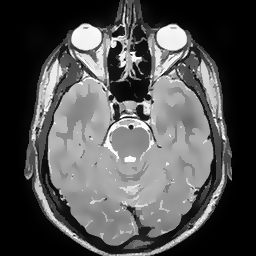
\includegraphics[width=.3\linewidth]{nld_100.png}}
\caption{Nonlinear diffusion filter. Contours are preserved.}
\label{fig:pde:matlab:nld}
\end{figure}

\subsection{Degenerate diffusion}

Erosion and dilation can theoretically be coded with this numerical scheme. However, some numerical problems appear in the first version (Fig.\ref{fig:pde:matlab:dd1}), which are corrected in the second version (Fig.\ref{fig:pde:matlab:dd2}).

\subsubsection{First version} 

This first version is the direct transcription of the numerical scheme. As observed in Fig.\ref{fig:pde:matlab:dd1}, shocks (peaks) appear after a few iterations.
\begin{matlab}
function [Zerosion,Zdilation] = morphologicalDiffusion2(I,nbIter,dt)
% I: original image
% nbIter: number of iterations
% dt: time increment
h = [-1 0 1];

Zerosion = I;
Zdilation = I;

for i=1:nbIter
    % calculate gradient in vertical V and horizontal H directions, for
    % dilation
    gH = imfilter(Zdilation, h);
    gV = imfilter(Zdilation, h');
    
    % same computation, for erosion
    jH = imfilter(Zerosion, h);
    jV = imfilter(Zerosion, h');
    
    % next step
    Zdilation  = Zdilation + dt * sqrt(gV.^2 +gH.^2);
    Zerosion = Zerosion - dt * sqrt(jV.^2 +jH.^2);

end
\end{matlab}


\begin{figure}[htbp]
 \centering
 \subfloat[Dilation by diffusion, for $dt=0.02$ and nbIter=20.]{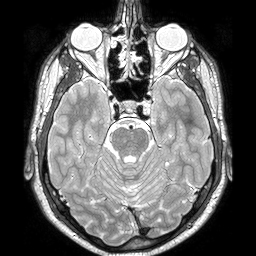
\includegraphics[width=.3\linewidth]{Idilshock20.png}}\hspace{1cm}
\subfloat[Dilation by diffusion, for $dt=0.02$ and nbIter=50.]{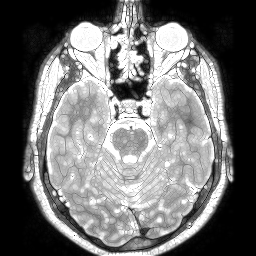
\includegraphics[width=.3\linewidth]{Idilshock50.png}}
\caption{Mathematical morphology operations by diffusion.}
\label{fig:pde:matlab:dd1}
\end{figure}


\subsubsection{More sophisticated version}

Another scheme, more numerically stable, can be preferred to the previous one.
Results are presented in Fig. \ref{fig:pde:matlab:dd2}.
\begin{matlab}
function [Zerosion,Zdilation] = morphologicalDiffusion(I,nbIter,dt)
% I: original image
% nbIter: number or iterations
% dt: time increment
hW = [1 -1 0];
hE = [0 -1 1];
hN = hW';
hS = hE';

Zerosion = I;
Zdilation = I;

for i=1:nbIter;
    % calculate gradient in all directions (N,S,E,W)
    gW = imfilter(Zdilation,hW);
    gE = imfilter(Zdilation,hE);
    gN = imfilter(Zdilation,hN);
    gS = imfilter(Zdilation,hS);
    
    jW = imfilter(Zerosion,hW);
    jE = imfilter(Zerosion,hE);
    jN = imfilter(Zerosion,hN);
    jS = imfilter(Zerosion,hS);
    
    % next step
    g = sqrt( min(0,-gW).^2 + max(0,gE).^2 + min(0,-gN).^2 + max(0,gS).^2 );
    j = sqrt( max(0,-jW).^2 + min(0,jE).^2 + max(0,-jN).^2 + min(0,jS).^2 );
    Zdilation = Zdilation + dt * g;
    Zerosion = Zerosion - dt * j;

end;
\end{matlab}

\begin{figure}[htbp]
 \centering
 \subfloat[Dilation by diffusion, for $dt=0.02$ and nbIter=20.]{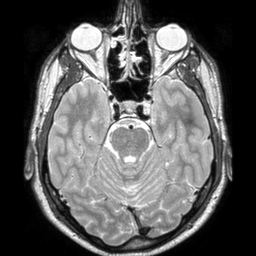
\includegraphics[width=.3\linewidth]{Idildiff20.png}}\hspace{1cm}
\subfloat[Dilation by diffusion, for $dt=0.02$ and nbIter=50.]{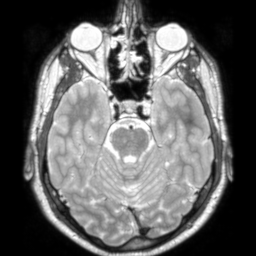
\includegraphics[width=.3\linewidth]{Idildiff50.png}}
\caption{Mathematical morphology operations by diffusion, sophisticated version.}
\label{fig:pde:matlab:dd2}
\end{figure}

